\documentclass[12pt,a4paper]{article}
\usepackage[utf8]{inputenc}
\usepackage[spanish,es-tabla]{babel}
\usepackage{geometry}
\usepackage{graphicx}
\usepackage{multirow}
\usepackage{tabularx}
\usepackage{mathptmx}
\usepackage{fancyhdr}
\usepackage{array}
\usepackage[table]{xcolor}
\usepackage{titlesec}
\usepackage{setspace}
\usepackage{microtype}
\usepackage{lastpage}
\usepackage{booktabs}
\usepackage{enumitem}
\usepackage{amsmath}
\usepackage{amsfonts}
\usepackage{amssymb}

\graphicspath{{images/}{../images/}{./}}

\geometry{
    top=4.7cm,
    bottom=2.5cm,
    left=2.5cm,
    right=2.5cm,
    headheight=3.9cm,
    headsep=0.4cm
}

\setstretch{1.15}
\setlength{\parindent}{0pt}
\setlength{\parskip}{0.45em}
\setlength{\tabcolsep}{4pt}

\titleformat{\section}
  {\normalfont\fontsize{12}{14.5}\bfseries}{\thesection.}{0.6em}{\uppercase}
\titlespacing*{\section}
  {0pt}{1.8ex plus 0.4ex minus 0.2ex}{0.6ex plus 0.2ex}

\titleformat{\subsection}
  {\normalfont\fontsize{11.5}{13.5}\bfseries}{\thesubsection.}{0.5em}{}
\titlespacing*{\subsection}
  {0pt}{1.4ex plus 0.3ex minus 0.1ex}{0.4ex plus 0.1ex}

\titleformat{\subsubsection}
  {\normalfont\fontsize{10.5}{12.5}\bfseries\itshape}{\thesubsubsection.}{0.4em}{}
\titlespacing*{\subsubsection}
  {0pt}{1.1ex plus 0.2ex minus 0.1ex}{0.3ex plus 0.1ex}

\newcolumntype{Y}{>{\centering\arraybackslash}X}
\newcolumntype{L}{>{\raggedright\arraybackslash}X}
\newcolumntype{C}{>{\centering\arraybackslash}X}

\definecolor{headerred}{RGB}{180, 0, 0}
\definecolor{darkred}{RGB}{140, 0, 0}
\definecolor{lightgraybg}{RGB}{248, 248, 248}
\definecolor{tableheader}{RGB}{232, 238, 246}

\newcommand{\docCodigo}{TI-SIGE-ENT-S1-003}
\newcommand{\docVersion}{1.0}
\newcommand{\docProceso}{INGENIERÍA DE REQUERIMIENTOS / ESPECIFICACIÓN}
\newcommand{\docElaboracion}{18/08/2026}
\newcommand{\docRevision}{PENDIENTE DE REVISIÓN}
\newcommand{\docTitulo}{ESPECIFICACIÓN DE REQUISITOS FUNCIONALES Y NO FUNCIONALES (IEEE 830)}
\newcommand{\docOrganizacion}{FACULTAD DE INGENIERÍA EN SISTEMAS, ELECTRÓNICA E INDUSTRIAL}
\newcommand{\docSubOrganizacion}{CARRERA DE INGENIERÍA DE SOFTWARE}

\newcommand{\encabezadofrecuente}{%
    \renewcommand{\arraystretch}{1.15}%
    \noindent\makebox[\textwidth][c]{%
    \begin{tabularx}{\textwidth}{|>{\centering\arraybackslash}m{2.8cm}|Y|>{\centering\arraybackslash}m{4.8cm}|}
        \hline
        \multirow{4}{2.8cm}{\centering\raisebox{-1.15cm}{
\includegraphics[width=2.5cm,height=2.0cm,keepaspectratio]{images/logo.png}}}
        & \textbf{\fontsize{9}{11}\selectfont \docOrganizacion} 
        & \textbf{\fontsize{8}{10}\selectfont CÓDIGO:} \fontsize{8}{10}\selectfont \docCodigo \\
        \cline{3-3}
        & \textbf{\fontsize{8.5}{10.5}\selectfont \docSubOrganizacion} 
        & \textbf{\fontsize{8}{10}\selectfont VERSIÓN:} \fontsize{8}{10}\selectfont \docVersion \\
        \cline{2-3}
        & \textbf{\fontsize{8}{10}\selectfont PROCESO:} \fontsize{8}{10}\selectfont \docProceso 
        & \textbf{\fontsize{8}{10}\selectfont ELABORACIÓN:} \fontsize{8}{10}\selectfont \docElaboracion \\
        \cline{2-3}
        & \textbf{\fontsize{8.5}{10.5}\selectfont \docTitulo} 
        & \textbf{\fontsize{8}{10}\selectfont ÚLTIMA REVISIÓN:} \fontsize{8}{10}\selectfont \textbf{\textcolor{darkred}{\docRevision}} \\
        \hline
    \end{tabularx}%
    }%
}

\pagestyle{fancy}
\fancyhf{}
\fancyhead[C]{\encabezadofrecuente}
\fancyfoot[C]{\fontsize{10}{12}\selectfont Página \thepage\ de \pageref{LastPage}}
\renewcommand{\headrulewidth}{0pt}

\begin{document}

\section{Título}
\textbf{Denominación del Entregable:} Especificación Formal de Requisitos del Sistema (SRS - IEEE 830)



\section{Introducción}
El presente documento formaliza la totalidad de los requerimientos del sistema \textbf{SIGE} siguiendo las directrices del estándar internacional \textbf{IEEE 830 (Software Requirements Specification)}. La especificación abarca la totalidad de operaciones necesarias para garantizar la digitalización de los formatos oficiales SGC (\texttt{UTA-SGC-A-2-1-P7-T1} y \texttt{UTA-SGC-A-2-1-P7-T2}), la validación determinista de matrices, el almacenamiento en la nube privada MinIO y la asistencia mediante IA local.

\section{Objetivo}

\subsection{Objetivo General}
Especificar de forma exhaustiva, verificable y no ambigua los 24 requisitos funcionales (RF-01 al RF-24) y los 8 requisitos no funcionales (RNF-01 al RNF-08) que rigen el comportamiento técnico del sistema SIGE.

\subsection{Objetivos Específicos}
\begin{itemize}[leftmargin=1.5em, itemsep=1.5pt, topsep=1.5pt]
    \item Detallar los 6 módulos funcionales: Seguridad/Roles, Encabezados/Autogeneración, Edición/Matrices SGC, Evidencias MinIO/IA, Firmas/Workflow y Seguimiento/Auditoría.
    \item Definir las métricas cuantitativas de aceptación para rendimiento, seguridad, disponibilidad y privacidad.
    \item Establecer la prioridad de implementación para los sprints de desarrollo.
\end{itemize}

\section{Alcance}

\subsection{Límites de la Especificación}
Define los requisitos de la aplicación web responsive SPA (React + Vite, Tailwind CSS Keyframes) y de la API REST modular backend (Node.js + Express v5, PostgreSQL 18, MinIO S3 y Google Gemini API).

\subsection{Exclusiones}
No incluye el desarrollo de aplicaciones nativas móviles (iOS/Android) durante la presente versión.

\section{Definiciones}
\begin{itemize}[leftmargin=1.5em, itemsep=2pt, topsep=2pt]
    \item \textbf{RF (Requisito Funcional):} Declaración de servicios o funciones que el software debe ejecutar obligatoriamente.
    \item \textbf{RNF (Requisito No Funcional):} Restricción de calidad técnica impuesta sobre el rendimiento, seguridad o arquitectura.
    \item \textbf{Deterministic Math Engine:} Módulo en memoria que recalcula subtotales y totales sin depender del almacenamiento en base de datos.
    \item \textbf{MinIO Object Storage:} Servidor de objetos compatible con Amazon S3 para gestión distribuida de archivos PDF/imágenes.
\end{itemize}

\section{Responsabilidades}
\begin{itemize}[leftmargin=1.5em, itemsep=2pt, topsep=2pt]
    \item \textbf{Analistas de Requerimientos (Heidy Villavicencio / Andrea Vásquez):} Redactar, numerar y validar la verificabilidad de los requisitos según IEEE 830.
    \item \textbf{Líder Técnico (Steeven Toala):} Asegurar la viabilidad técnica y compatibilidad de los RNF con la arquitectura de microservicios.
\end{itemize}

\section{Normativa Legal y Técnica}
\begin{itemize}[leftmargin=1.5em, itemsep=2pt, topsep=2pt]
    \item \textbf{IEEE Std 830-1998:} Recommended Practice for Software Requirements Specifications.
    \item \textbf{ISO/IEC/IEEE 29148:2018:} Systems and software engineering -- Life cycle processes -- Requirements engineering.
    \item \textbf{OWASP ASVS 4.0:} Application Security Verification Standard (Nivel 2).
\end{itemize}

\section{Método, Políticas y Contenidos}

\subsection{Desglose Modular de Requisitos Funcionales}
Los 24 requerimientos se estructuran en 6 paquetes funcionales críticos:

\begin{figure}[htbp]
    \centering
    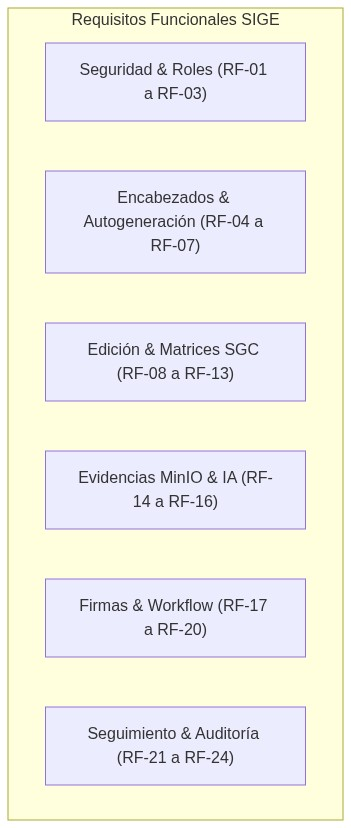
\includegraphics[width=0.55\textwidth,height=7.5cm,keepaspectratio]{images/s1_03_modulos_rf.png}
    \caption{Desglose Modular de Requisitos Funcionales del Sistema SIGE.}
    \label{fig:s1_03_rf_modulos}
\end{figure}

\section{Descripción de actividades}

A continuación, se detalla el catálogo completo de los **24 Requisitos Funcionales (RF-01 al RF-24)** organizados por módulos temáticos, seguido del catálogo de los **8 Requisitos No Funcionales (RNF-01 al RNF-08)**:

\subsection{Módulo 1: Seguridad, Roles y Encabezados (RF-01 a RF-07)}
\begin{table}[htbp]
\centering
\small
\begin{tabularx}{\textwidth}{|>{\hsize=0.35\hsize\bfseries\centering\arraybackslash}X|>{\hsize=0.85\hsize\bfseries}X|>{\hsize=1.5\hsize}X|>{\hsize=0.3\hsize\centering\arraybackslash}X|}
    \hline
    \rowcolor{tableheader}
    Código & Nombre del Requisito & Descripción Detallada & Prioridad \\
    \hline
    RF-01 & Autenticación Segura y JWT & El sistema debe permitir el inicio de sesión institucional mediante credenciales seguras y emisión de JSON Web Tokens (JWT). & ALTA \\
    \hline
    RF-02 & Control de Acceso por Roles (RBAC) & El sistema debe restringir vistas y acciones según el rol asignado (\textit{Elaborador, Revisor, Validador, Aprobador, Administrador}). & ALTA \\
    \hline
    RF-03 & Gestión de Perfil de Usuario & El sistema debe permitir consultar los datos del usuario, carrera asignada y firma digital registrada. & MEDIA \\
    \hline
    RF-04 & Autodetección de Período Académico & El sistema debe autodetectar y fijar el período académico oficial (\textit{Julio-Diciembre o Enero-Junio}) sin intervención manual. & ALTA \\
    \hline
    RF-05 & Fechas Autogeneradas Inmutables & Las fechas de emisión, envío y actualización deben ser generadas por el servidor, impidiendo su edición manual. & ALTA \\
    \hline
    RF-06 & Codificación Única de Documentos & El sistema debe generar la nomenclatura institucional oficial (ej. \texttt{SOFT-JD2026-INF-042-V01}). & ALTA \\
    \hline
    RF-07 & Índices de Contenido y Tablas & El sistema debe compilar automáticamente el índice de contenido y de tablas a partir de las secciones del documento. & MEDIA \\
    \hline
\end{tabularx}
\caption{Requisitos Funcionales del Módulo 1 (RF-01 al RF-07).}
\label{tab:s1_03_rf_m1}
\end{table}

\subsection{Módulo 2: Edición Modular y Matrices SGC (RF-08 a RF-13)}
\begin{table}[htbp]
\centering
\small
\begin{tabularx}{\textwidth}{|>{\hsize=0.35\hsize\bfseries\centering\arraybackslash}X|>{\hsize=0.85\hsize\bfseries}X|>{\hsize=1.5\hsize}X|>{\hsize=0.3\hsize\centering\arraybackslash}X|}
    \hline
    \rowcolor{tableheader}
    Código & Nombre del Requisito & Descripción Detallada & Prioridad \\
    \hline
    RF-08 & Wizard Modular de Edición & La interfaz debe guiar la redacción mediante pestañas ordenadas: Datos Generales, Antecedentes, Matriz, Conclusiones, Gestiones y Firmas. & ALTA \\
    \hline
    RF-09 & Editor de Texto Enriquecido TipTap & El sistema debe incorporar un editor enriquecido con soporte para listas, tablas, negrita y autoguardado asíncrono (\textit{debounce}). & ALTA \\
    \hline
    RF-10 & Catálogo de Actividades en BD & El sistema debe cargar las actividades planificadas desde un combo administrable en BD según el área institucional. & ALTA \\
    \hline
    RF-11 & Llenado Estricto de Matriz & El sistema no debe permitir añadir una nueva fila hasta que la fila actual tenga actividad, fechas, medios y \% de avance completo. & ALTA \\
    \hline
    RF-12 & Justificación de Desvío ($<100\%$) & Si el porcentaje de ejecución de una actividad es menor al $100\%$, el campo de observaciones de desvío es obligatorio. & ALTA \\
    \hline
    RF-13 & Cálculo Automático de Ponderaciones & El sistema debe validar en tiempo real que la suma de ponderaciones de la matriz sea estrictamente igual al $100\%$. & ALTA \\
    \hline
\end{tabularx}
\caption{Requisitos Funcionales del Módulo 2 (RF-08 al RF-13).}
\label{tab:s1_03_rf_m2}
\end{table}

\subsection{Módulo 3: Evidencias MinIO, Asistente y Firmas (RF-14 a RF-20)}
\begin{table}[htbp]
\centering
\small
\begin{tabularx}{\textwidth}{|>{\hsize=0.35\hsize\bfseries\centering\arraybackslash}X|>{\hsize=0.85\hsize\bfseries}X|>{\hsize=1.5\hsize}X|>{\hsize=0.3\hsize\centering\arraybackslash}X|}
    \hline
    \rowcolor{tableheader}
    Código & Nombre del Requisito & Descripción Detallada & Prioridad \\
    \hline
    RF-14 & Almacenamiento Evidencias MinIO S3 & El sistema debe almacenar archivos adjuntos (PDFs, imágenes) en un bucket privado de MinIO mediante URLs prefirmadas. & ALTA \\
    \hline
    RF-15 & Asistente Ortográfico Local & El sistema debe ofrecer corrección ortográfica y gramatical asíncrona conectándose a un contenedor Docker local de LanguageTool. & MEDIA \\
    \hline
    RF-16 & Registro de Contactos y Delegaciones & El sistema debe proveer una tabla específica para registrar instituciones, temas tratados y compromisos de comisiones oficiales. & MEDIA \\
    \hline
    RF-17 & Circuito Secuencial de Firmas & El flujo de legalización debe exigir la firma del Elaborador $\rightarrow$ Revisor $\rightarrow$ Validador/Aprobador en estricto orden. & ALTA \\
    \hline
    RF-18 & Observaciones del Revisor & El revisor debe poder emitir observaciones por párrafo y registrar dictamen (\textit{Aprobado, Observado, Rechazado}). & ALTA \\
    \hline
    RF-19 & Rechazo y Retorno a Borrador & Si un informe es rechazado, el sistema debe devolverlo a estado borrador para corrección e incrementar la versión (\texttt{V02}). & ALTA \\
    \hline
    RF-20 & Historial de Cambios y Versionado & El sistema debe registrar la versión autoincremental, fecha del sistema y descripción obligatoria del cambio. & ALTA \\
    \hline
\end{tabularx}
\caption{Requisitos Funcionales del Módulo 3 (RF-14 al RF-20).}
\label{tab:s1_03_rf_m3}
\end{table}

\subsection{Módulo 4: Seguimiento, Reportes y Auditoría (RF-21 a RF-24)}
\begin{table}[htbp]
\centering
\small
\begin{tabularx}{\textwidth}{|>{\hsize=0.35\hsize\bfseries\centering\arraybackslash}X|>{\hsize=0.85\hsize\bfseries}X|>{\hsize=1.5\hsize}X|>{\hsize=0.3\hsize\centering\arraybackslash}X|}
    \hline
    \rowcolor{tableheader}
    Código & Nombre del Requisito & Descripción Detallada & Prioridad \\
    \hline
    RF-21 & Seguimiento en Tiempo Real & El sistema debe permitir a los revisores validar avances intermedios y calificar evidencias durante la vigencia del plan. & ALTA \\
    \hline
    RF-22 & Pre-carga Automática del Informe & Al generar el Informe de Cumplimiento, el sistema debe pre-cargar las actividades, \% y evidencias auditadas del Plan de Trabajo. & ALTA \\
    \hline
    RF-23 & Exportación Oficial Word y PDF & El sistema debe exportar documentos idénticos al formato oficial SGC en \texttt{.pdf} (QuestPDF) y \texttt{.docx} (OpenXML). & ALTA \\
    \hline
    RF-24 & Auditoría Inmutable SHA-256 & El sistema debe registrar cada cambio de estado con timestamp, IP de origen, usuario y hash criptográfico. & ALTA \\
    \hline
\end{tabularx}
\caption{Requisitos Funcionales del Módulo 4 (RF-21 al RF-24).}
\label{tab:s1_03_rf_m4}
\end{table}

\subsection{Catálogo Completo de Requisitos No Funcionales (RNF-01 al RNF-08)}
\begin{table}[htbp]
\centering
\small
\begin{tabularx}{\textwidth}{|>{\hsize=0.35\hsize\bfseries\centering\arraybackslash}X|>{\hsize=0.65\hsize\bfseries}X|>{\hsize=1.0\hsize}X|>{\hsize=1.0\hsize}X|}
    \hline
    \rowcolor{tableheader}
    Código & Categoría & Requisito No Funcional & Métrica de Aceptación \\
    \hline
    RNF-01 & Seguridad & Cifrado de contraseñas con Bcrypt.js, autenticación basada en JWT, cabeceras HTTP reforzadas con Helmet, protección contra inyecciones SQL y sanitización XSS. & Cumplimiento de estándares OWASP Top 10. \\
    \hline
    RNF-02 & Rendimiento & Tiempo de respuesta de endpoints de consulta y guardado en la API REST de Express (v5). & Menor a 500 ms bajo carga normal (50 usuarios concurrentes). \\
    \hline
    RNF-03 & Disponibilidad & Tiempo de actividad continuo del sistema en servidor VPS. & Disponibilidad mínima del $99.5\%$ en horario académico. \\
    \hline
    RNF-04 & Usabilidad & Diseño institucional en paleta \texttt{\#00345E} (Azul UTA / FISEI) con Tailwind CSS + CSS Keyframes para animaciones fluidas por GPU y navegación SPA en React + Vite. & Cero saturación visual; reducción de errores de digitación en un $80\%$. \\
    \hline
    RNF-05 & Privacidad y Eficiencia IA & El módulo de IA debe proteger la privacidad académica y operar sin suscripciones de pago. & Corrección ortográfica 100\% local en Docker (LanguageTool); sugerencias semánticas vía Google Gemini API. \\
    \hline
    RNF-06 & Compatibilidad & Soporte para navegadores modernos de escritorio y dispositivos móviles. & Chrome $\ge$ 110, Firefox $\ge$ 115, Edge $\ge$ 110 y Safari $\ge$ 16. \\
    \hline
    RNF-07 & Mantenibilidad & Arquitectura modular en capas basada en Node.js + Express (v5) (\texttt{modules/auth}, \texttt{modules/users}, middlewares y controladores) con código limpio y pruebas automatizadas. & Cobertura de pruebas unitarias $> 80\%$ en lógica de negocio. \\
    \hline
    RNF-08 & Integridad de Datos & Persistencia relacional ACID en PostgreSQL (18) mediante scripts DDL (\texttt{schema.sql}, \texttt{seed.sql}, \texttt{init.js}) y respaldo periódico de base de datos y MinIO. & RPO $< 24$ horas, RTO $< 2$ horas ante fallos catastróficos. \\
    \hline
\end{tabularx}
\caption{Catálogo de Requisitos No Funcionales (RNF-01 al RNF-08).}
\label{tab:s1_03_rnf_completo}
\end{table}

% =============================================================
% 10. FIRMAS DE RESPONSABILIDAD
% =============================================================
\section{Firmas de Responsabilidad}

\noindent
\renewcommand{\arraystretch}{1.2}
\begin{tabularx}{\textwidth}{|>{\raggedright\arraybackslash}m{2.9cm}|>{\raggedright\arraybackslash}X|>{\centering\arraybackslash}m{4.6cm}|>{\centering\arraybackslash}m{2.3cm}|}
    \hline
    \rowcolor{headerred}
    \textcolor{white}{\textbf{ACCIÓN}} & \textcolor{white}{\textbf{NOMBRE Y CARGO}} & \textcolor{white}{\textbf{FIRMA}} & \textcolor{white}{\textbf{FECHA}} \\
    \hline
    \textbf{Elaborado por:} & Heidi Villavicencio\newline \textit{Analista de Requerimientos / UI-UX} & \parbox[c]{4.4cm}{\centering\vspace{4pt}
\includegraphics[height=1.5cm,width=4.0cm,keepaspectratio]{images/firma_heidi.png}\vspace{4pt}} & 18/08/2026 \\
    \hline
    \textbf{Revisado por:} & Steeven Toala\newline \textit{Líder de Proyecto / Arquitecto Software} & \parbox[c]{4.4cm}{\centering\vspace{10pt}\textbf{\textcolor{gray!80}{\scriptsize [ PENDIENTE DE REVISIÓN ]}}\vspace{10pt}} & \textbf{\textcolor{gray!90}{Pendiente}} \\
    \hline
    \textbf{Aprobado por:} & Ing. Paulo Torres\newline \textit{Docente Tutor - Gestión Proyectos Software} & \parbox[c]{4.4cm}{\centering\vspace{10pt}\textbf{\textcolor{gray!80}{\scriptsize [ PENDIENTE DE APROBACIÓN ]}}\vspace{10pt}} & \textbf{\textcolor{gray!90}{Pendiente}} \\
    \hline
\end{tabularx}

\vspace{0.4cm}

% =============================================================
% 11. CONTROL DE CAMBIOS
% =============================================================
\section{Control de Cambios}

\noindent
\renewcommand{\arraystretch}{1.2}
\begin{tabularx}{\textwidth}{|>{\hsize=0.45\hsize\centering\arraybackslash}X|>{\hsize=1.55\hsize\raggedright\arraybackslash}X|>{\hsize=1.2\hsize\raggedright\arraybackslash}X|>{\hsize=0.8\hsize\centering\arraybackslash}X|}
    \hline
    \rowcolor{gray!20}
    \textbf{Versión} & \textbf{Descripción del cambio} & \textbf{Responsable del cambio} & \textbf{Fecha de aprobación} \\
    \hline
    1.0 & Especificación formal completa de requisitos funcionales (RF-01 al RF-24) y no funcionales (RNF-01 al RNF-08) IEEE 830 / Pendiente de revisión & Heidi Villavicencio & \textbf{\textcolor{gray!90}{Pendiente de Revisión}} \\
    \hline
\end{tabularx}

\vspace{0.4cm}

\section{Anexos}
\subsection*{Anexo 1: Matriz de Trazabilidad entre Requisitos Funcionales y Casos de Uso}
Mapeo formal de los 24 requerimientos funcionales hacia los 16 casos de uso parametrizados en la Semana 2.

\end{document}



